\documentclass[sigconf]{acmart}
\setcopyright{none}
\settopmatter{printfolios=true}

\usepackage{fontspec}
\setmonofont[Scale=0.88]{Iosevka}
\newfontfamily\emoji{DejaVu Sans}

\usepackage{csquotes}
\usepackage{minted}
\usepackage{subcaption}
\usepackage{wasysym}
\usepackage{pgfplots}
\usepackage{enumitem}

\urlstyle{tt}

\begin{document}

\title{\vspace{-0.5em}{\hspace{-5.5cm}\small \textsc{SQL is a Programming Language}}\\\vspace{-0.3em}Handwriting Recognition with SQL\\\vspace{-0.1em}\hspace{6.88cm}\footnotesize and a tiny bit of web stuff\vspace{-1em}}
\author{Noah Doersing}
\affiliation{}
\email{noah.doersing@student.uni-tuebingen.de}

\maketitle

\section*{Abstract}
A basic handwriting recognition algorithm conceived in the 60's has been implemented, 50 years later, on top of a modern relational database system. We discuss the origins of the system, introduce the algorithm and its SQL implementation, provide a web app that captures pen strokes and sends them off to the database for processing, evaluate the approach and provide further context.

\section{Introduction}

Throughout the history of computing, human-computer interaction has been an ever-evolving avenue for research. The results of computations, in the early days indicated by blinking light bulbs, have more recently been presented on screens of ever-increasing resolution, with different output formats being explored continuously. On the input side of the equation, punch cards have given way to command prompts fed by keyboards, which in turn have largely been superseded by touch- or voice-based user interfaces.

Both need to operate in lockstep: The meshing of input and output methods must be carefully considered if an interface is to feel natural to its users. Today's touch-based input devices, when compared to now-old-fashioned mouse input, exhibit clear usability upsides – when the user wishes to manipulate a thing, she can simply touch it, instead of negotiating a mouse pointer towards it or entering keyboard shortcuts.

\textit{Current} as this may be, it is not fundamentally \textit{new}. More than 50 years ago, researchers at RAND Corporation came up with a pen-based input paradigm intended, according to GUI pioneer Alan Kay, \enquote{for economists and other non-computer specialists [...] who said \enquote{Hey, none of us can type, can't you do something about that?}} \cite{kay} As part of this system, a basic handwriting recognition algorithm was developed. \cite{groner,schaedler}

\textbf{Outline.} Before delving into its details – and how a simplified variant of it, only able to recognize a single-stroke letter at a time (see figure \ref{chars}), has been implemented as a SQL query – we will take a look at the RAND tablet and the GRAIL system it powers. After discussing the implementation, we will consider its performance and some related ideas.

\begin{figure}[pb]
  \centering
  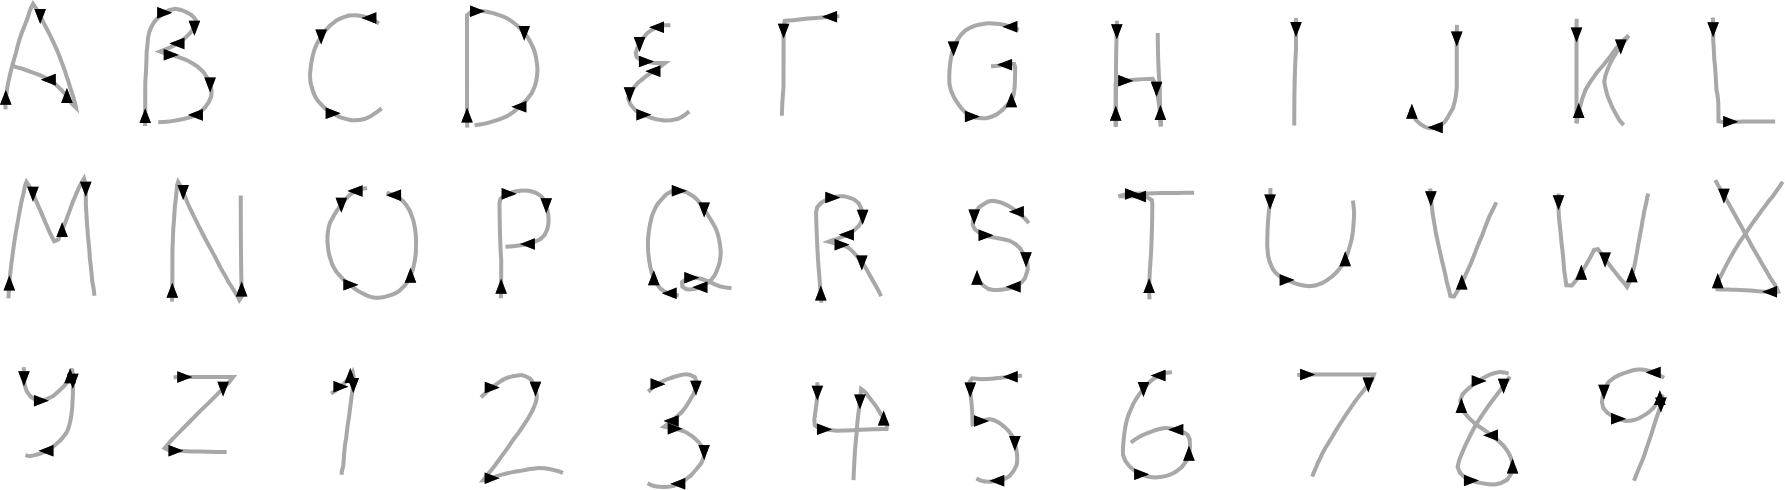
\includegraphics[width=7cm]{drawingguide}
  \caption{How to draw the simplified characters.}
  \label{chars}
\end{figure}

\section{GRAIL and the RAND tablet}

\begin{figure}[tpb]
  \centering
  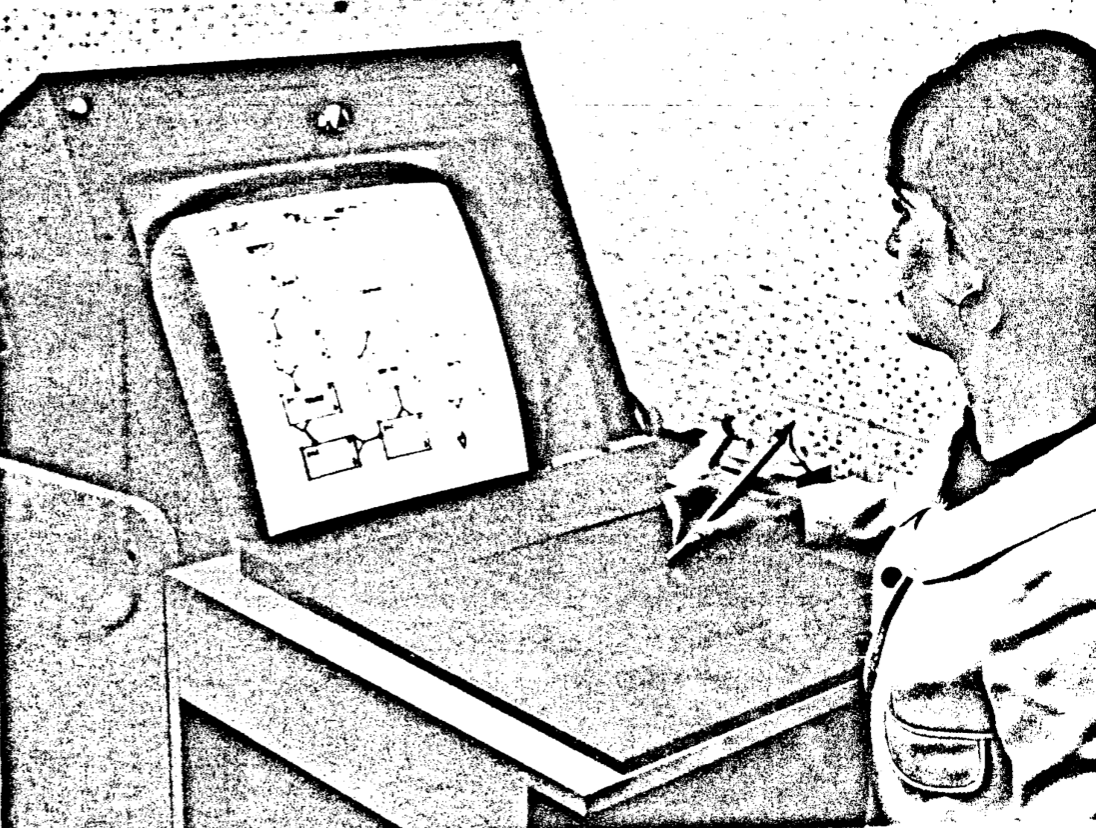
\includegraphics[width=7cm]{grailconsole}
  \caption{A scan \cite{grail} of a printout of a photograph of a user interacting with GRAIL.}
  \label{grailconsole}
\end{figure}

Developed at RAND in the 1960s, the Graphic Input Language (GRAIL) was a flowchart-based programming system \cite{kay,grailang,grail}. As described by its creators, it enables a user to \enquote{draw flowchart symbols, edit and rearrange them on the display surface, and connect them appropriately to form a meaningful program. [The user can] execute the program while controlling its execution rate and the amount and content of information presented to him. The system interprets, in real-time, the [user's] hand-drawn figures, characters, and other [...] gestures to provide germane responses on the display surface.} \cite{grailang} Alan Kay, in a talk where he demonstrates GRAIL, summarizes it as \enquote{the world's first modeless system}
%and notes that it is \enquote{where Macintosh window control came from}
\cite{kay}.

The user operated the GRAIL system using a stylus connected to a tablet as shown in figure \ref{grailconsole}. Its \enquote{writing surface is a 10"x10" area with a resolution of 100 lines per inch in both x and y [...], allowing the user to \enquote{write} in a natural manner. [...] To maintain \enquote{naturalness} of the pen device, a pressure-sensitive switch in the tip of the stylus indicates \enquote{stroke} [...] to the computer} \cite{tablet}.\footnote{The authors of this memo describe the function of the tablet in great detail. Another memo takes a deep dive into the innards of GRAIL. \cite{details}}

The original \enquote{IBM/360 assembly language program for online graphical-input character recognition using the RAND Tablet} \cite{source} is publicly available, but was not consulted when writing the SQL query – it is too low-level to be of much utility.

\subsection{Web App}

Testing the SQL query necessitates a simple simulation of the RAND tablet, which was given along with the assignment in the form of a D3.js-based web app that prints a list of coordinates once the user draws a character.

In order to present the algorithm succinctly, this was extended with a server component that, with the help of some Python code, dynamically executes the handwriting recognition query on a Postgres instance and returns the result to the user.\footnote{This is given in \texttt{code/index.html}. The backend setup is a can of worms, so it's recommended to just use the frontend, which yields a JSON version of the pen stroke.}

\begin{figure}[tpb]
  \centering
  \setminted{fontsize=\fontsize{6.04}{5.2}, linenos}
  \begin{minted}{sql}
WITH RECURSIVE
tablet(pos, x, y) -- ... (conversion of JSON list to rows)
smooth(pos, x, y) AS (
  SELECT pos, x :: real, y :: real FROM tablet WHERE pos = 1
    UNION ALL
  SELECT t.pos,
         (:smoothingfactor * s.x + (1.0 - :smoothingfactor) * t.x) :: real AS x,
         (:smoothingfactor * s.y + (1.0 - :smoothingfactor) * t.y) :: real AS y
  FROM   smooth s, tablet t
  WHERE  t.pos = s.pos + 1
),
thin(pos, x, y) AS (
  SELECT * FROM smooth WHERE pos = 1
    UNION ALL
  SELECT *
  FROM   (
    SELECT s.pos, s.x, s.y
    FROM   thin t, smooth s
    WHERE  s.pos > t.pos
    AND    :thinningsize < |/ (s.x - t.x)^2 + (s.y - t.y)^2
    ORDER BY s.pos
    LIMIT 1
  ) AS _
),
curve(pos, x, y, direction) AS (
  SELECT pos, x, y,
         COALESCE(degrees(-atan2( y - lag(y) OVER (ORDER BY pos),
                                 -x + lag(x) OVER (ORDER BY pos))
                         ) + 180, 90)
  FROM   thin
),
cardinal(pos, direction) AS (
  SELECT pos,
         (enum_range(NULL :: cardinal_direction))[(direction / 90) :: int % 4 + 1]
  FROM   curve
),
cardinal_change(pos, direction) AS (
  SELECT pos, direction
  FROM   (SELECT pos, direction,
                 COALESCE(lag(direction, 2) OVER win <> lag(direction) OVER win,
                          true)
                 AND lag(direction) OVER win = direction
          FROM cardinal
          WINDOW win AS (ORDER BY pos)) AS _(pos, direction, is_new)
  WHERE  is_new
),
corner(pos, x, y) AS (
  SELECT pos, x, y
  FROM   (SELECT pos, x, y, (
                   angdiff(lag(direction, 2) OVER win, lag(direction) OVER win) < 22.5
                   AND angdiff(lag(direction) OVER win, direction) > :cornerangle
                   AND angdiff(direction, lead(direction) OVER win) < 22.5
                 ) OR (  -- Immediate direction change OR one-segment turn.
                   angdiff(lag(direction, 3) OVER win, lag(direction, 2) OVER win) < 22.5
                   AND angdiff(lag(direction, 2) OVER win, direction) > :cornerangle
                   AND angdiff(direction, lead(direction) OVER win) < 22.5
                 ) AS is_corner
          FROM   curve
          WINDOW win AS (ORDER BY pos)) AS _(pos, x, y, is_corner)
  WHERE  is_corner
),
aabb(xmin, xmax, ymin, ymax, aspect, width, height, centerx, centery) -- ...
start_grid(n) AS (
  SELECT gridpos(a.width, a.height, a.xmin, a.ymin, s.x, s.y)
  FROM   smooth s, aabb a
  ORDER BY s.pos
  LIMIT 1
),
stop_grid(n) -- ... (analogous to start_grid)
corner_grid(pos, n) -- ... (also similar)
features(directions, start, stop, corners, width, height, aspect, center) AS (
  SELECT (SELECT array_agg(direction ORDER BY pos)
          FROM   cardinal_change),
         (TABLE start_grid),
         (TABLE stop_grid),
         (SELECT COALESCE(array_agg(n ORDER BY pos), '{}')
          FROM   corner_grid),
         width, height, aspect, point(centerx, centery)
  FROM   aabb
),
character(character) AS (
  SELECT l.character
  FROM   features f, lookup_candidates c, lookup_bestfit l
  WHERE  f.directions[1:4] = c.first_four_directions
  AND    c.candidate_characters = l.candidate_characters
  AND    (l.start IS NULL          OR f.start = l.start)
  AND    (l.stop IS NULL           OR f.stop = l.stop)
  AND    (l.corners IS NULL        OR f.corners = l.corners)
  AND    (l.aspect_range IS NULL   OR l.aspect_range @> f.aspect :: numeric)
)
TABLE character;
  \end{minted}
  \caption{Slightly condensed SQL implementation. Some custom functions have been omitted.}
  \label{code}
\end{figure}

\section{Implementation}

The web app outputs a JSON value of the form \texttt{[\{"x": 37, "y": 39\}, \{"x": 38, "y": 43, ...\}]}. It is passed to the Postgres\footnote{Postgres 9.4 or newer is required.} command-line client \texttt{psql} and converted to a table with a sequential identifier column in CTE \texttt{tablet} (see figure \ref{code}).

\subsection{Smoothing \& Thinning}

\begin{figure}[pb]
  \centering
  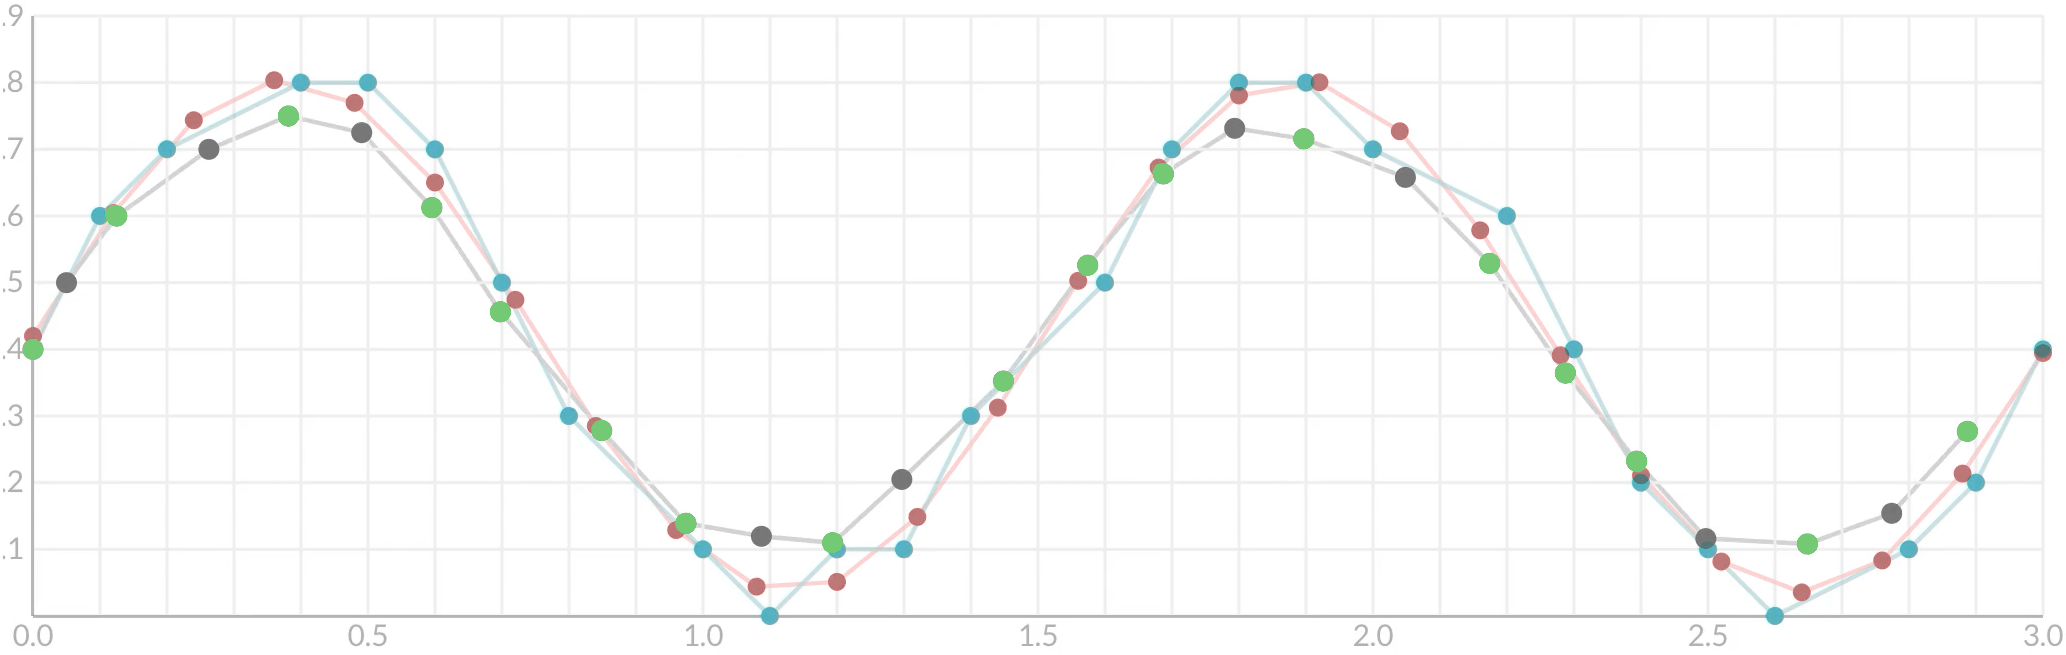
\includegraphics[width=8.6cm]{smoothingthinning}
  \caption{The {\color[HTML]{BE7777}\huge\textbullet} pen stroke drawn by the user, the corresponding {\color[HTML]{52B1C6}\huge\textbullet} quantized signal received by the computer, the {\color[HTML]{777777}\huge\textbullet} smoothed intermediate result and {\color[HTML]{74C974}\huge\textbullet} the points left after thinning.}
  \label{smoothingthinning}
\end{figure}

The RAND tablet provides a stream (\enquote{the recognition scheme is notified of [the pen] position every 4 msec} \cite{groner}) of pen positions as integer-valued $x,y$ coordinate pairs.

As a preprocessing step, this digital representation of the pen stroke is smoothed to counteract quantization effects (\enquote{noise due to the discreteness of the pen location as measured by the tablet} \cite{groner}, which can negatively affect the latter steps of the algorithm) as shown in figure \ref{smoothingthinning}. Smoothing is performed by computing a weighted average of the most recently smoothed point (weight ~75\%; the first point of the stroke is accepted as is) and the next incoming point (~25\%). In SQL, this is accomplished by the recursive CTE \texttt{smooth} where the weight is read from the \texttt{psql} variable \texttt{smoothingfactor}.

The second stage of preprocessing, thinning, drops points that are in close proximity to the most recently accepted point and thus contribute little or no additional information. This mainly serves to ease the computing effort required during the next steps. Groner uses a set of inequalities that compare $x$ and $y$ positions, effectively superimposing a square over each thinned point (again, the first point is accepted as is) and removing any other points that fall into this square. This is less \enquote{correct} than pruning based on the Euclidean distance as implemented in the SQL query (line 20), but computationally more efficient. The seemingly superfluous wrapping of the recursive part of the \texttt{thin} CTE in a \texttt{SELECT * FROM (...) AS \_} is required because Postgres does not permit \texttt{ORDER BY} directly in a recursive query.

The degree to which these steps affect the raw data is controlled using the \texttt{psql} variables \texttt{smoothingfactor} and \texttt{thinningsize}. Choosing sensible values is crucial: As \texttt{smoothingfactor} approaches 1, corners disappear and the end of the stroke is pulled closer to the start. This effect is visible in figure \ref{smoothingthinning} where {\color[HTML]{BE7777}\huge\textbullet}{\color[HTML]{52B1C6}\huge\textbullet} extend further along the $x$ axis than {\color[HTML]{777777}\huge\textbullet}{\color[HTML]{74C974}\huge\textbullet}. Similarly, a large \texttt{thinningsize} can obscure corners or bends, which character recognition hinges on.

\subsection{Curvature}

\enquote{Curvature is the most obvious characteristic which is independent of position and size, and yet which describes the [stroke]'s shape. [...] Four directions, used in conjunction with other features, provide sufficient description for recognition, yet result in [less effort] than do [more] directions.} \cite{groner} The algorithm only keeps \textit{changes} of these cardinal directions the pen stroke moves toward as each character is drawn.

Groner extracts this feature by comparing positional differences of point pairs using a set of inequalities. Because more fine-grained curvature information is helpful in detecting corners later on, the SQL implementation (see CTE \texttt{curve}) instead computes the precise angle between the imaginary line segment connecting each pair of points and the $x$ axis as shown in figure \ref{tan}.

\begin{figure}[htpb]
  \centering
  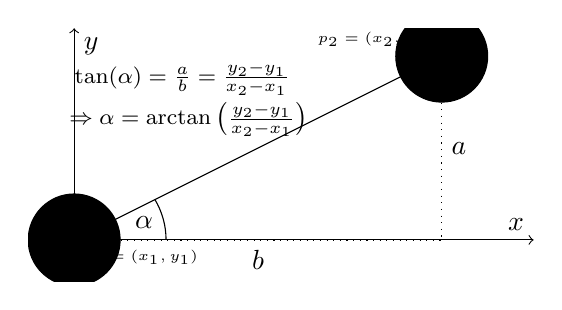
\begin{tikzpicture}
    \begin{axis}[
      ticks=none,
      axis lines = center,
      axis line style={->},
      ymin=-0.6, ymax=4.3,
      xmin=-1, xmax=10,
      axis equal,
      xlabel=$x$, ylabel=$y$,
      height=4.8cm,width=8cm]
      \addplot[black, domain=0:8] {x*0.5};
      \draw[black,fill=black] (axis cs:0,0) circle [radius=1] node[below right]{\tiny $p_1 = (x_1,y_1)$};
      \draw[black,fill=black] (axis cs:8,4) circle [radius=1]  node[above left]{\tiny $p_2 = (x_2,y_2)$};
      \draw (axis cs:2,0) arc[radius=1cm,start angle=0,end angle=31] node[left,yshift=-0.3cm,xshift=0.1cm]{$\alpha$} node[above,xshift=0.35cm,yshift=1.2cm]{\footnotesize$\tan(\alpha) = \frac{a}{b} = \frac{y_2-y_1}{x_2-x_1}$} node[below,xshift=0.43cm,yshift=1.35cm]{\footnotesize$\Rightarrow \alpha = \arctan\left(\frac{y_2-y_1}{x_2-x_1}\right)$};
      \draw[dotted] (axis cs:8,4) -- node[right]{$a$} (axis cs:8,0);
      \draw[dotted] (axis cs:0,-.02) -- node[below]{$b$} (axis cs:8,-.02);
    \end{axis}
  \end{tikzpicture}
  \caption{Deriving the angle $\alpha$ between two points $p_1$ and $p_2$.}
  \label{tan}
\end{figure}

In CTE \texttt{cardinal} $\alpha$ is then quantized to determine the cardinal directions, denoted by an \texttt{ENUM} type containing the Unicode symbols $\blacktriangle\hspace{-0.15em}\blacktriangledown\hspace{-0.45em}\blacktriangleleft\blacktriangleright$. To accomplish this, the \texttt{enum\_range(anyenum)} function, which returns all values of the input enum type as an array, is used.\footnote{See \url{https://www.postgresql.org/docs/8.3/static/functions-enum.html}.}

As mentioned above, \enquote{[i]f the same direction occurs twice in succession, and is not the same as the last direction [...], then it is added to the [result], otherwise it is discarded} \cite{groner}, which the CTE \texttt{cardinal\_change} takes care of. Because window functions cannot\footnote{\enquote{This is because they logically execute after the processing of [this clause]}, see \url{https://www.postgresql.org/docs/10/static/tutorial-window.html}.} be used in \texttt{WHERE} predicates, an somewhat awkward subquery builds a boolean column, based on which the rows are then filtered (lines 39 to 45).

\begin{figure}[pb]
  \centering
  \subcaptionbox{Corners help discern between similar characters. They are determined based on the angles between four to five successive line segments.\label{corners}}{
    \includegraphics[height=3.9cm]{corners}
  }
  \hspace{0.5cm}
  \subcaptionbox{The absolute positions of corners, as well as start and end of a stroke are converted to grid positions.\label{grid}}{
    \hspace{0.4cm}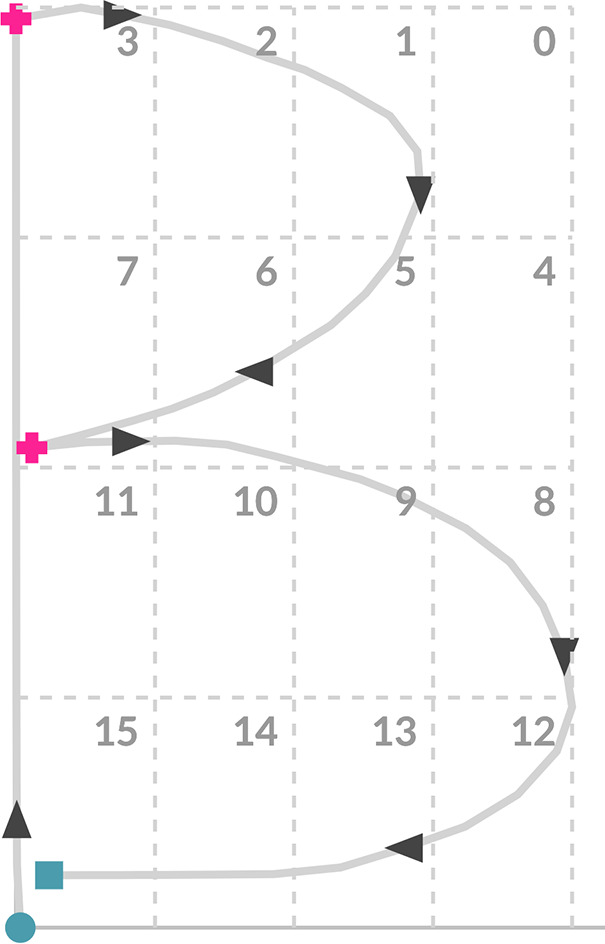
\includegraphics[height=3.9cm]{grid}\hspace{0.4cm}
  }
  \caption{Cardinal directions, corners and the grid.}
  \label{cornergrid}
\end{figure}

\subsection{Corners}

Cardinal directions are sufficient to discern between many characters, but in some cases, \textit{e.g.}, G and 6 as demonstrated in figure \ref{corners}, other features such as the presence or absence of corners are required. \enquote{A corner is detected whenever the pen moves in the same ($\pm 1$) 16-direction for at least two segments [{\color[HTML]{21C800}$\blacktriangleright\blacktriangleright$}], changes direction by at least 90°, and then proceeds along the new direction ($\pm 1$) for at least two segments [{\color[HTML]{008AFF}$\blacktriangleright\blacktriangleright$}]. The change in direction must take place either immediately or through a one-segment turn [{\color[HTML]{FFC000}$\blacktriangleright$}].} \cite{groner} (The triangles correspond to the lower half of figure \ref{corners}.)

Instead of 16-directions (\textit{i.e.}, the division of 360° into 16 slices), the CTE \texttt{corner} of the SQL implementation uses absolute angles, making sure that the angles corresponding to the two line segments directly before a corner are within $\frac{360°}{16} = 22.5°$ of each other, the angle at the corner point is $>90°$ and the two subsequent angles again differ by no more than $22.5°$. The window function \texttt{lag()} is used to access these previous and next angles and a custom \texttt{angdiff()} function computes the delta $$\arctan\left(\frac{\sin(\alpha-\beta)}{\cos(\alpha-\beta)}\right)$$ between each pair of angles.\footnote{See \url{https://stackoverflow.com/a/2007279}. The formula $180 - \left|\left|\alpha - \beta\right| - 180\right|$ is equivalent and cheaper to compute, but the one given in the text elegantly combines sin, cos and (arc)tan.} The output of the CTE is a table of corner positions.

\subsection{Additional Features}

In addition to cardinal directions and corners, Groner's algorithm determines a number of additional features: \enquote{the symbol's height and width [...], its aspect ratio [...], and its center relative to the tablet origin.} \cite{groner} They are of limited use to the simplified single-stroke alphanumeric characters recognized by the SQL implementation; \textit{e.g.}, height and width help discern parentheses from commata, neither of which are supported.

Nevertheless, they are extracted in the CTE \texttt{aabb}, which trivially derives an axis-aligned bounding box around the character drawn by the user and returns two $x,y$ coordinates defining it, along with width, height, center and aspect ratio.

\textbf{Grid.} The algorithm then \enquote{divides the rectangular area defined by the symbol into a 4 x 4 grid. The starting (pen-down) and ending (pen-up) points, as well as the corner locations, are then each encoded as lying in one of these 16 areas, thereby locating them relative to the symbol.} \cite{groner} Figure \ref{grid} shows an example.

The SQL implementation uses a custom \texttt{gridpos(width, height, xmin, ymin, x, y)} function which \enquote{desugars} to an arithmetic expression mapping \texttt{x} and \texttt{y}, given an AABB defined by minimum x, y, width and height to one of the 16 grid positions.\footnote{Global state would be convenient here to avoid passing the unchanging AABB on each call, but creating an extra temporary table for storing it seems like overkill.}

Finally, the CTE \texttt{features} combines all extracted features into a handy single-row table.

\subsection{Mapping Features to Characters}

Once the pen stroke has been sufficiently analyzed, Groner's algorithm \enquote{[looks] up the first four direction segments} in a table. For the letter B as shown in figure \ref{grid}, this table entry is $\blacktriangle\hspace{-0.26em}\blacktriangleright\hspace{-0.40em}\blacktriangledown\hspace{-0.40em}\blacktriangleleft$, which corresponds to 2, 3, 8, B, D, P, or R. \enquote{Further tests, based on this particular set of possibilities, result in a single identification.} \cite{groner}

In the original implementation, these tests take the form of a custom decision tree for each entry of the initial lookup table. A direct transliteration to SQL is difficult, requiring a rat's tail of nested \texttt{CASE} expressions or a similarly convoluted approach. However, the simplified alphabet used in the context of this work suggested a more idiomatic two-stage approach that, while less flexible, delivers acceptable results:

\begin{enumerate}[nolistsep]
    \item An array comprising the first four cardinal directions is mapped to an array of possible characters using lookup table $T_1$.
    \item Another lookup table $T_2$ is consulted, mapping the potential characters and specific feature values – some of which can be marked as \enquote{don't care} by setting them to \texttt{NULL}, hence the \texttt{IS NULL} checks in lines 86 through 89 – to a concrete result character. For characters which are wholly determined by the first lookup, all features are set to \texttt{NULL}.
\end{enumerate}

Finding a satisfactory representation for this decision mechanism was one of the trickier aspects of this work: A reasonable balance between flexibility and maintainability needed to be struck while ideally still resembling Groner's ideas.

\textbf{Alternate approach.} The two-stage approach implemented in CTE \texttt{character} is not ideal: The array-to-array mapping of $T_1$ does not conform to 1NF. An alternate representation\footnote{Its implementation can be found in the \texttt{morerelational} branch of the Git repository.} was explored where the rows of $T_1$ were \enquote{expanded} to map to single characters from direction arrays (which can now occur multiple times in the table) and $T_2$ is modified accordingly by chopping off the array column. This, however, complicates the CTE \texttt{character} and complicates future expansion \textit{and} discerning some pairs of characters: Deciding whether a stroke resembles 7 or 1 requires different features than the choice between 7 and 3, say. This difficulty, however, could be patched over on the query level.

%TODO benjamin's idea worse because
%* 4-direction patterns in the first lookup table that map to a *single* character essentially skip the second lookup table (see `INSERT` in line 116 of the setup file). This could be somehow emulated using a query (if `COUNT(candidate\_character)` for the current pattern is 1, skip the feature-matching step), but that adds cruft to the query.
%* Deciding between 7 and 1 requires features F, while deciding between 7 and 3 requires looking at features G != F. Could also be patched over at the query level.
%* More verbose first lookup table, slimmer second lookup table.
%* Second lookup table does not anymore indicate which 4-direction pattern a given feature match belongs to, making debugging/extending harder.
%* Effectively requires ranking results based on closeness of match, e.g. number of features used (or VERY careful design of the second lookup table, which I didn't have time for before my presentation).
%* Conceptually further from original tree structure, which can be a bad or good thing.

\section{Evaluation}

Basing his analysis on the original IBM/360 assembly program running on a Model 40, Groner writes that the preprocessing and feature extraction stage \enquote{takes up about 40 percent of the available computing time in the limiting case [...]. Smoothing and thinning requires about 20 percent of this analysis time, [drawing each incoming segment to the screen] 30 percent, and corner detection 16 percent. The remainder of the analysis time is for computing quantized directions, updating x and y extremes, and bookkeeping.} He goes on to outline potential improvements that could cut the computing time down to \enquote{only about 15 percent} \cite{groner} but does not mention the cost of walking the decision tree – supposedly it's minimal. Groner also presents the results of user testing.

The SQL implementation takes $10-15$ ms to process a typical pen stroke generated by the web app. Taking a look at the output of \texttt{EXPLAIN ANALYZE}, none of the CTEs take an unexpectedly high amount of \texttt{actual time}. Thus, the computing effort seems to be relatively evenly spread, without any major departures from Groner's observations.

\section{Related \& future work}

\textbf{Related work.} GRAIL is a successor to Sketchpad, one of the first systems that \enquote{[make] it possible for a man and a computer to converse rapidly through the medium of line drawings} but relied on a keyboard for text input. \cite{sketchpad}

Because Chinese and Korean characters are drawn based on a rigidly defined stroke order, algorithms like the one presented are well-suited for these writing systems. Indeed, Groner and Heafner worked on \enquote{classification of handprinted Chinese characters as a translation aid} \cite{chinese} in the same timeframe.

Palm, Inc. later developed Graffiti, a text input system based on single-stroke characters and commands. Among other devices, it was deployed on Apple's Newton and Windows Mobile.\footnote{See \url{https://en.wikipedia.org/wiki/Graffiti_(Palm_OS)}.} The SQL implementation could conceivably be modified to recognize Graffiti's gestures by rewriting the lookup tables.

DTW may be used for handwriting recognition, contingent on an effective way of converting pen strokes to time series.\footnote{Ask the guy in B312 about this. {\emoji 😉}}

Jack Schaedler has build an excellent \textit{explorable explanation} \cite{schaedler} showcasing GRAIL's handwriting recognition scheme, which many visualizations used in this work are based on.

\textbf{Future work.} Recognizing characters composed of multiple strokes would bring the SQL implementation to basic feature parity with the original system.

Groner's decision tree could be represented more effectively – building the character recognition scheme on top of a graph database \textit{might} lend itself to an implementation that's more true to the original.

Because modern tablets feature resolutions significantly higher than the RAND tablet, the smoothing step is less crucial now than it was back then. Similarly, the time savings brought about by thinning barely make a dent on modern systems.

\bibliographystyle{abbrv}
\bibliography{paper.bib}


\end{document}
